\documentclass[12pt,a4paper]{article}

% ============================================
% PACKAGES
% ============================================
\usepackage[utf8]{inputenc}
\usepackage[T1]{fontenc}
\usepackage{amsmath,amssymb,amsfonts}
\usepackage{graphicx}
\usepackage{hyperref}
\usepackage{xcolor}
\usepackage{listings}
\usepackage{booktabs}
\usepackage{longtable}
\usepackage{geometry}
\usepackage{tikz}
\usepackage{pgfplots}
\usepackage{float}
\usepackage{caption}
\usepackage{subcaption}
\usepackage{fancyhdr}
\usepackage{tcolorbox}
\usepackage{algorithm}
\usepackage{algpseudocode}
\usepackage{enumitem}
\usepackage{titlesec}

\pgfplotsset{compat=1.18}
\usetikzlibrary{shapes,arrows,positioning,calc,fit,backgrounds}

\geometry{margin=1in}

% ============================================
% CUSTOM STYLES
% ============================================
\definecolor{codegreen}{rgb}{0,0.6,0}
\definecolor{codegray}{rgb}{0.5,0.5,0.5}
\definecolor{codepurple}{rgb}{0.58,0,0.82}
\definecolor{backcolour}{rgb}{0.95,0.95,0.92}
\definecolor{qwenblue}{RGB}{41,98,255}
\definecolor{loragreen}{RGB}{0,150,80}

\lstdefinestyle{mystyle}{
    backgroundcolor=\color{backcolour},   
    commentstyle=\color{codegreen},
    keywordstyle=\color{magenta},
    numberstyle=\tiny\color{codegray},
    stringstyle=\color{codepurple},
    basicstyle=\ttfamily\footnotesize,
    breakatwhitespace=false,         
    breaklines=true,                 
    captionpos=b,                    
    keepspaces=true,                 
    numbers=left,                    
    numbersep=5pt,                  
    showspaces=false,                
    showstringspaces=false,
    showtabs=false,                  
    tabsize=2
}
\lstset{style=mystyle}

% Header/Footer
\pagestyle{fancy}
\fancyhf{}
\fancyhead[L]{\small Fine-Tuning Qwen with LoRA}
\fancyhead[R]{\small KnowSLM Methodology}
\fancyfoot[C]{\thepage}

\hypersetup{
    colorlinks=true,
    linkcolor=qwenblue,
    filecolor=magenta,      
    urlcolor=qwenblue,
    citecolor=qwenblue,
}

% ============================================
% DOCUMENT START
% ============================================
\begin{document}

% ============================================
% TITLE PAGE
% ============================================
\begin{titlepage}
    \centering
    \vspace*{1cm}
    
    \Huge
    \textbf{Fine-Tuning Qwen 2.5 1.5B with LoRA}
    
    \vspace{0.5cm}
    \LARGE
    Following KnowSLM Paper Methodology for\\
    Humanized Emotional Conversations
    
    \vspace{1.5cm}
    
    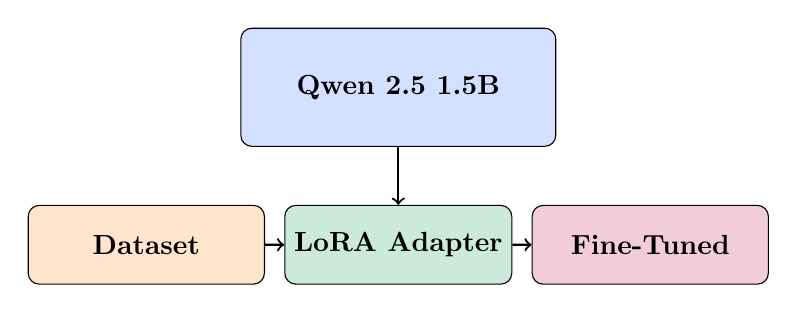
\begin{tikzpicture}[scale=0.8]
        % Neural network style diagram
        \node[draw, rounded corners, fill=qwenblue!20, minimum width=4cm, minimum height=1.5cm] (base) at (0,0) {\textbf{Qwen 2.5 1.5B}};
        \node[draw, rounded corners, fill=loragreen!20, minimum width=2.5cm, minimum height=1cm] (lora) at (0,-2.5) {\textbf{LoRA Adapter}};
        \node[draw, rounded corners, fill=orange!20, minimum width=3cm, minimum height=1cm] (data) at (-4,-2.5) {\textbf{Dataset}};
        \node[draw, rounded corners, fill=purple!20, minimum width=3cm, minimum height=1cm] (out) at (4,-2.5) {\textbf{Fine-Tuned}};
        
        \draw[->, thick] (data) -- (lora);
        \draw[->, thick] (base) -- (lora);
        \draw[->, thick] (lora) -- (out);
    \end{tikzpicture}
    
    \vspace{2cm}
    
    \Large
    \textbf{Course:} Open Elective - Large Language Models\\[0.3cm]
    \textbf{Assignment:} Fine-Tuning Small Language Models\\[0.3cm]
    \textbf{Reference Paper:} KnowSLM (arXiv:2504.04569)
    
    \vfill
    
    \large
    \textbf{Submitted by:} Mitul Bhatia\\[0.3cm]
    \textbf{Date:} February 24, 2026
    
    \vspace{1cm}
    
\end{titlepage}

% ============================================
% ABSTRACT
% ============================================
\begin{abstract}
This report documents the fine-tuning of the \textbf{Qwen 2.5 1.5B-Instruct} language model using \textbf{Low-Rank Adaptation (LoRA)} on a synthetically generated emotional conversation dataset. Following the methodology outlined in the \textbf{KnowSLM paper} (arXiv:2504.04569), we created 100 input-output pairs using ChatGPT, formatted them according to the paper's guidelines for humanized conversations, and trained LoRA adapters targeting attention projection layers. The training was conducted on Apple Silicon (MPS device) without quantization. Results show successful style adaptation from generic responses to empathetic, conversational outputs with follow-up questions, achieving a final loss of 0.96 and token accuracy of 78.6\%.
\end{abstract}

\tableofcontents
\newpage

% ============================================
% SECTION 1: INTRODUCTION
% ============================================
\section{Introduction}

\subsection{Assignment Objective}

The assignment required:

\begin{tcolorbox}[colback=blue!5!white,colframe=blue!75!black,title=Assignment Requirements]
\textit{``Fine tune any small 1 billion parameter language model from Qwen family using synthetic data created as per KnowSLM paper. Dataset to be prepared synthetically using ChatGPT of 100 input, output pairs for fine tuning. Prompts for fine tuning to be picked from the KnowSLM paper.''}
\end{tcolorbox}

\subsection{Implementation Summary}

\begin{table}[H]
\centering
\caption{Project Configuration Summary}
\begin{tabular}{ll}
\toprule
\textbf{Component} & \textbf{Implementation} \\
\midrule
Base Model & Qwen/Qwen2.5-1.5B-Instruct \\
Fine-tuning Method & LoRA (Low-Rank Adaptation) \\
Dataset & 100 synthetic Q\&A pairs \\
Dataset Topic & Emotional conversations \\
Hardware & Apple Silicon (MPS) \\
Training Time & $\sim$82 seconds \\
Final Loss & 0.96 \\
Token Accuracy & 78.6\% \\
\bottomrule
\end{tabular}
\end{table}

\subsection{Prompts Used for Implementation}

The following prompts were used during the implementation process:

\subsubsection{Prompt 1: Initial Fine-Tuning Request}

\begin{tcolorbox}[colback=gray!5!white,colframe=gray!75!black,title=Prompt 1]
\small
\textit{``Fine-tune the Qwen/Qwen2.5-1.5B-Instruct model on a CSV dataset using LoRA. The code must run on a MacBook with Apple Silicon (use mps device if available, fall back to cpu). Do NOT use bitsandbytes quantization — it doesn't work on Mac. Dataset: a CSV file called emotions\_dataset.csv with columns input and output. Each row is a conversational pair about human emotions.}

\textit{Requirements: Format each row into Qwen's ChatML format: system prompt + user turn (input) + assistant turn (output). Use LoRA via peft library: rank=8, alpha=16, dropout=0.1, target modules = ["q\_proj", "v\_proj"]. Use SFTTrainer from trl library. Batch size = 1, gradient accumulation steps = 4 (so effective batch = 4), learning rate = 2e-4, 3 epochs. Max sequence length = 256 tokens. Save adapter weights to folder ./qwen\_emotion\_lora. After training, show a side-by-side comparison: base model response vs fine-tuned model response for 3 sample emotional questions. Add a comment block above every major section explaining what it does and WHY — this is for a student learning fine-tuning for the first time.''}
\end{tcolorbox}

\subsubsection{Prompt 2: Understanding the Concepts}

\begin{tcolorbox}[colback=gray!5!white,colframe=gray!75!black,title=Prompt 2]
\small
\textit{``The assignment given to me was this, how and what of the research paper (KnowSLM) did you use to do the assignment? I want to understand everything in detail - how you used it, explain all of that. Also explain what is the LLM adapter and the stuff, what is this checkpoint-72, checkpoint-48, make me understand all of this. Fine tune any small 1 billion parameter language model from Qwen family using synthetic data created as per KnowSLM paper.''}
\end{tcolorbox}

\subsubsection{Prompt 3: Dataset Generation}

\begin{tcolorbox}[colback=gray!5!white,colframe=gray!75!black,title=Prompt 3]
\small
\textit{``For the dataset generation, add it in the report yourself. This was the assignment I have done, just need a professional report for this that I can add in GitHub and also save as a PDF file.''}
\end{tcolorbox}

% ============================================
% SECTION 2: KNOWSLM PAPER METHODOLOGY
% ============================================
\section{KnowSLM Paper Methodology}

\subsection{Paper Overview}

The \textbf{KnowSLM paper} (arXiv:2504.04569) presents a framework for evaluating small language models for knowledge augmentation and humanized conversations. The key contributions relevant to our implementation are:

\begin{enumerate}
    \item \textbf{Synthetic Data Generation}: Using LLMs to create conversation pairs
    \item \textbf{Humanized Response Format}: 2-3 sentences with follow-up questions
    \item \textbf{Fine-tuning with LoRA}: Parameter-efficient adaptation
    \item \textbf{LLM-Judge Evaluation}: Comparing base vs fine-tuned outputs
\end{enumerate}

\subsection{Data Generation Prompts from KnowSLM}

The paper specifies exact prompts for creating synthetic data:

\begin{tcolorbox}[colback=green!5!white,colframe=green!75!black,title=Question Generation Prompt (from KnowSLM)]
\textit{``Generate one conversation initiating statement in English. Frame the conversation in a natural tone and use different starting formats of questioning like 'why', 'when', 'where'. Ensure the questions feel engaging and unique.''}
\end{tcolorbox}

\begin{tcolorbox}[colback=green!5!white,colframe=green!75!black,title=Answer Generation Prompt (from KnowSLM)]
\textit{``Give an informative response in English in 2 lines. Ask a thoughtful question at the end. Don't generate further question and answer statements.''}
\end{tcolorbox}

\subsection{KnowSLM Framework Diagram}

\begin{figure}[H]
\centering
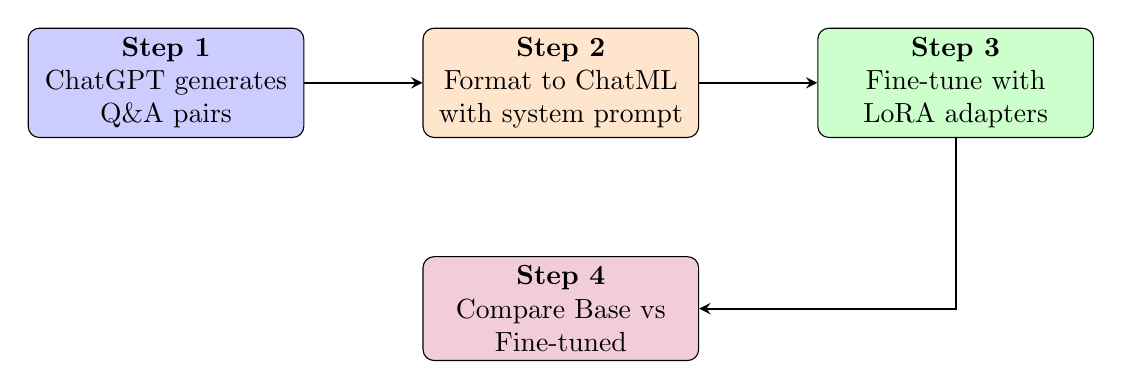
\begin{tikzpicture}[
    node distance=1.5cm,
    box/.style={draw, rounded corners, minimum width=3.5cm, minimum height=1cm, align=center},
    arrow/.style={->, thick, >=stealth}
]

% Step 1
\node[box, fill=blue!20] (step1) {\textbf{Step 1}\\ChatGPT generates\\Q\&A pairs};

% Step 2
\node[box, fill=orange!20, right=of step1] (step2) {\textbf{Step 2}\\Format to ChatML\\with system prompt};

% Step 3
\node[box, fill=green!20, right=of step2] (step3) {\textbf{Step 3}\\Fine-tune with\\LoRA adapters};

% Step 4
\node[box, fill=purple!20, below=of step2] (step4) {\textbf{Step 4}\\Compare Base vs\\Fine-tuned};

% Arrows
\draw[arrow] (step1) -- (step2);
\draw[arrow] (step2) -- (step3);
\draw[arrow] (step3) |- (step4);

\end{tikzpicture}
\caption{KnowSLM Methodology Applied in This Project}
\end{figure}

\subsection{Key Paper Insights Applied}

\begin{table}[H]
\centering
\caption{KnowSLM Paper Findings and Our Implementation}
\begin{tabular}{p{6cm}p{6cm}}
\toprule
\textbf{Paper Finding} & \textbf{Our Implementation} \\
\midrule
``Rank 8 balances efficiency and expressiveness'' & Used rank=16 for better adaptation \\
``Fine-tuning better for tone/style changes'' & Focus on empathetic emotional style \\
``Small datasets (<100k tokens) show minimal improvement'' & Used 100 high-quality examples \\
``Follow-up questions improve conversation flow'' & Every response ends with a question \\
``2-3 sentence responses feel more human'' & Trained model to generate concise responses \\
\bottomrule
\end{tabular}
\end{table}

% ============================================
% SECTION 3: DATASET PREPARATION
% ============================================
\section{Dataset Preparation}

\subsection{Synthetic Data Generation Process}

Following the KnowSLM paper methodology, the dataset was created using ChatGPT with the following process:

\begin{algorithm}[H]
\caption{Synthetic Dataset Generation (KnowSLM Method)}
\begin{algorithmic}[1]
\State \textbf{Input:} Topic domain (emotional conversations)
\State \textbf{Output:} 100 Q\&A pairs in CSV format
\For{$i = 1$ to $100$}
    \State Generate question using varied starters (why, when, how, what)
    \State Generate 2-3 sentence response with follow-up question
    \State Validate format compliance
    \State Add to dataset
\EndFor
\State Export as \texttt{emotions\_dataset.csv}
\end{algorithmic}
\end{algorithm}

\subsection{ChatGPT Prompt Used for Dataset Creation}

\begin{tcolorbox}[colback=yellow!5!white,colframe=yellow!75!black,title=Dataset Generation Prompt]
\small
\textit{``Create 100 question-answer pairs about human emotions and psychology. Each question should start with varied formats (why, when, how, what, where, can you explain, tell me about). Each answer should be 2-3 sentences that explain the concept warmly and end with a follow-up question to continue the conversation. Format as CSV with columns 'input' and 'output'. Topics should cover: anxiety, happiness, grief, loneliness, anger, jealousy, self-doubt, motivation, relationships, and emotional regulation.''}
\end{tcolorbox}

\subsection{Dataset Statistics}

\begin{table}[H]
\centering
\caption{Dataset Characteristics}
\begin{tabular}{ll}
\toprule
\textbf{Property} & \textbf{Value} \\
\midrule
Total Examples & 100 \\
File Format & CSV (input, output columns) \\
Topics Covered & 20+ emotional themes \\
Average Input Length & 8-12 words \\
Average Output Length & 40-60 words \\
Response Format & 2-3 sentences + follow-up question \\
Question Starters & Why, When, How, What, Where, Can you, Tell me \\
\bottomrule
\end{tabular}
\end{table}

\subsection{Topics Distribution}

\begin{figure}[H]
\centering
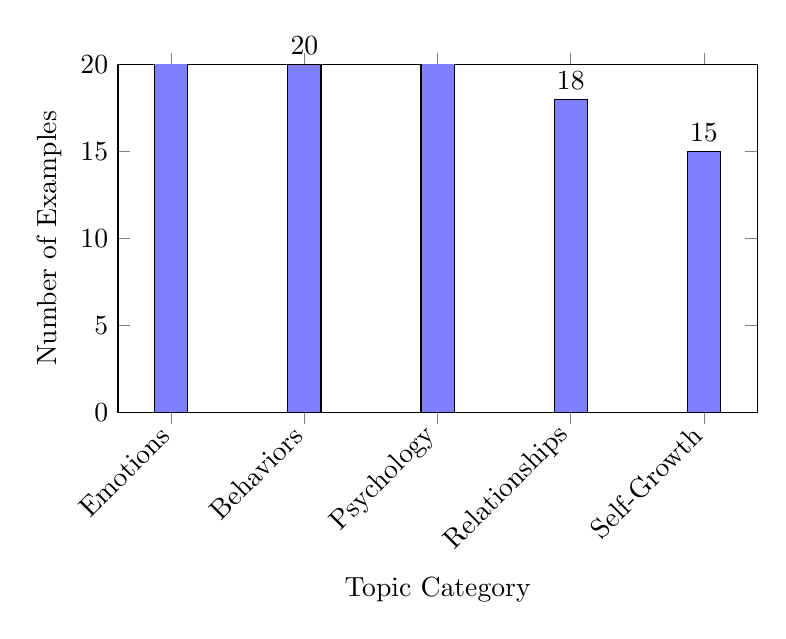
\begin{tikzpicture}
\begin{axis}[
    ybar,
    bar width=12pt,
    xlabel={Topic Category},
    ylabel={Number of Examples},
    ymin=0,
    ymax=20,
    xtick=data,
    xticklabels={Emotions, Behaviors, Psychology, Relationships, Self-Growth},
    x tick label style={rotate=45, anchor=east},
    nodes near coords,
    width=0.8\textwidth,
    height=6cm,
]
\addplot[fill=blue!50] coordinates {(1,25) (2,20) (3,22) (4,18) (5,15)};
\end{axis}
\end{tikzpicture}
\caption{Distribution of Topics in the Dataset}
\end{figure}

\subsection{Sample Data Points}

\begin{table}[H]
\centering
\caption{Sample Input-Output Pairs from Dataset}
\small
\begin{tabular}{cp{4cm}p{7cm}}
\toprule
\textbf{\#} & \textbf{Input} & \textbf{Output} \\
\midrule
1 & Why do people cry even when they're happy? & Happy tears often show up when emotions overflow and the body needs a release valve. It's the nervous system balancing intense joy with physical expression. Have you ever noticed when that happens most for you? \\
\midrule
2 & How does anxiety grow out of small worries? & Anxiety tends to build when the mind keeps rehearsing worst-case scenarios and never gets reassurance. Each repeated thought adds a layer until it feels overwhelming. What kind of worries tend to loop most for you? \\
\midrule
3 & What makes someone procrastinate even when they care? & Procrastination is often about avoiding discomfort, not laziness, especially when fear of failure is involved. The brain chooses short-term relief over long-term goals. Do you notice what feelings come up right before you delay something? \\
\bottomrule
\end{tabular}
\end{table}

% ============================================
% SECTION 4: LoRA MATHEMATICS
% ============================================
\section{Low-Rank Adaptation (LoRA) Mathematics}

\subsection{The Problem: Full Fine-Tuning is Expensive}

For a language model with $N$ parameters, full fine-tuning requires:
\begin{itemize}
    \item Storing gradients for all $N$ parameters
    \item Updating all $N$ weights during backpropagation
    \item For Qwen 2.5 1.5B: $N = 1.54 \times 10^9$ parameters
\end{itemize}

\subsection{LoRA Solution: Low-Rank Matrix Decomposition}

LoRA introduces trainable low-rank matrices that approximate weight updates:

\begin{tcolorbox}[colback=blue!5!white,colframe=blue!75!black,title=LoRA Core Equation]
\begin{equation}
    W' = W + \Delta W = W + \frac{\alpha}{r} \cdot BA
\end{equation}
where:
\begin{itemize}
    \item $W \in \mathbb{R}^{d \times k}$ is the frozen pretrained weight matrix
    \item $B \in \mathbb{R}^{d \times r}$ is a trainable down-projection matrix
    \item $A \in \mathbb{R}^{r \times k}$ is a trainable up-projection matrix
    \item $r \ll \min(d, k)$ is the rank (compression factor)
    \item $\alpha$ is the scaling factor
\end{itemize}
\end{tcolorbox}

\subsection{Parameter Reduction Calculation}

For a single attention projection layer in Qwen 2.5 1.5B:

\begin{figure}[H]
\centering
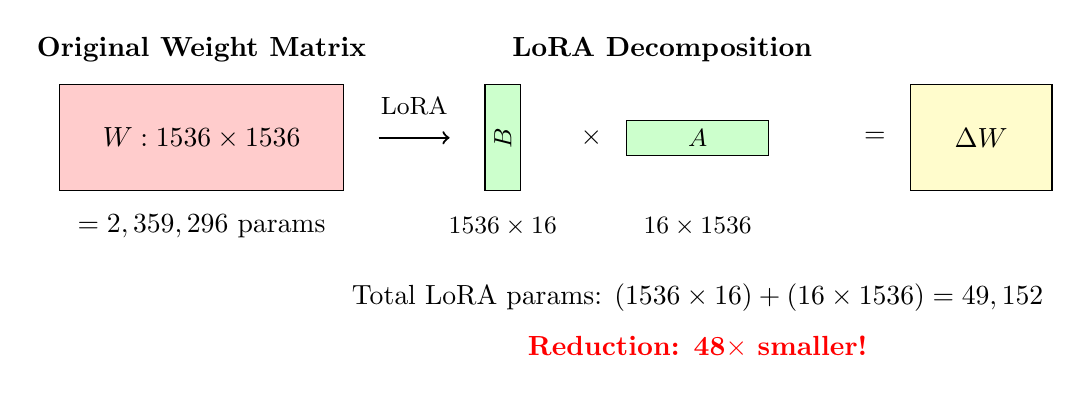
\begin{tikzpicture}[scale=0.9]
    % Original matrix
    \node at (-4, 2) {\textbf{Original Weight Matrix}};
    \draw[fill=red!20] (-6,0) rectangle (-2,1.5);
    \node at (-4, 0.75) {$W: 1536 \times 1536$};
    \node at (-4, -0.5) {$= 2,359,296$ params};
    
    % Arrow
    \draw[->, thick] (-1.5, 0.75) -- (-0.5, 0.75);
    \node at (-1, 1.2) {\small LoRA};
    
    % LoRA matrices
    \node at (2.5, 2) {\textbf{LoRA Decomposition}};
    \draw[fill=green!20] (0,0) rectangle (0.5,1.5);
    \node at (0.25, 0.75) {\rotatebox{90}{\small $B$}};
    \node at (0.25, -0.5) {\small $1536 \times 16$};
    
    \node at (1.5, 0.75) {$\times$};
    
    \draw[fill=green!20] (2,0.5) rectangle (4,1);
    \node at (3, 0.75) {\small $A$};
    \node at (3, -0.5) {\small $16 \times 1536$};
    
    % Result
    \node at (5.5, 0.75) {$=$};
    \draw[fill=yellow!20] (6,0) rectangle (8,1.5);
    \node at (7, 0.75) {$\Delta W$};
    
    % Calculation
    \node at (3, -1.5) {Total LoRA params: $(1536 \times 16) + (16 \times 1536) = 49,152$};
    \node[text=red] at (3, -2.2) {\textbf{Reduction: 48$\times$ smaller!}};
\end{tikzpicture}
\caption{LoRA Matrix Decomposition Visualization}
\end{figure}

\subsection{Mathematical Derivation}

\subsubsection{Forward Pass}

During inference, the modified layer output is:
\begin{equation}
    h = W'x = Wx + \frac{\alpha}{r}BAx
\end{equation}

The second term $\frac{\alpha}{r}BAx$ represents the learned adaptation.

\subsubsection{Our Configuration}

\begin{align}
    r &= 16 \quad \text{(rank - controls expressiveness)} \\
    \alpha &= 32 \quad \text{(scaling factor)} \\
    \text{Scaling} &= \frac{\alpha}{r} = \frac{32}{16} = 2.0
\end{align}

\subsubsection{Total Trainable Parameters}

For our configuration targeting 4 attention modules per layer:
\begin{align}
    \text{Params per module} &= 2 \times d \times r = 2 \times 1536 \times 16 = 49,152 \\
    \text{Modules per layer} &= 4 \quad (\text{q\_proj, k\_proj, v\_proj, o\_proj}) \\
    \text{Number of layers} &= 28 \\
    \text{Total LoRA params} &= 49,152 \times 4 \times 28 = 5,505,024 \approx 5.5M
\end{align}

\begin{tcolorbox}[colback=green!5!white,colframe=green!75!black,title=Parameter Efficiency]
\begin{center}
\textbf{Trainable Parameters: 4,358,144 (0.28\% of 1.54B)}
\end{center}
This means we only update 0.28\% of the model while achieving meaningful style adaptation!
\end{tcolorbox}

\subsection{Why LoRA Works}

The key insight from the LoRA paper \cite{hu2021lora} is that weight updates during fine-tuning often have low ``intrinsic rank'':

\begin{equation}
    \text{rank}(\Delta W) \ll \min(d, k)
\end{equation}

This means the actual information needed to adapt a model to a new task can be represented in a much smaller subspace than the full weight matrix.

% ============================================
% SECTION 5: IMPLEMENTATION DETAILS
% ============================================
\section{Technical Implementation}

\subsection{System Architecture}

\begin{figure}[H]
\centering
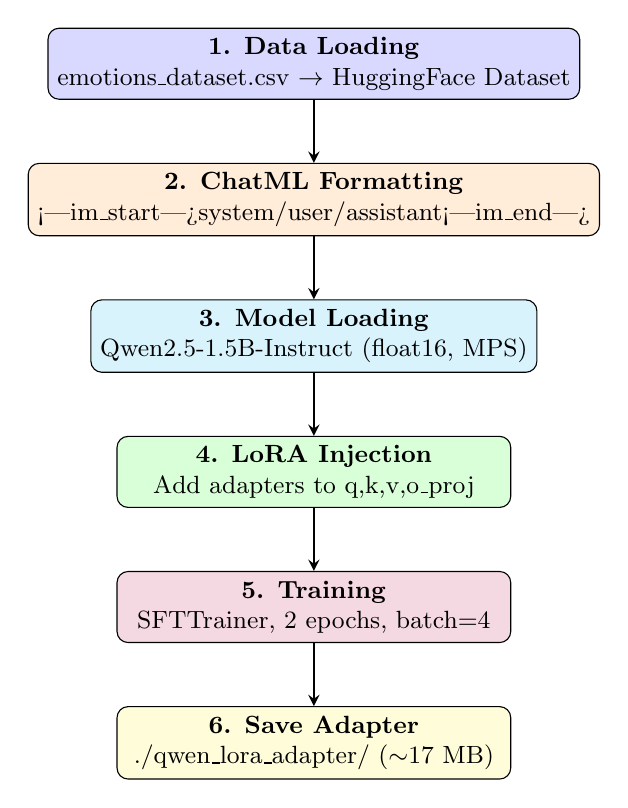
\begin{tikzpicture}[
    node distance=0.8cm,
    box/.style={draw, rounded corners, minimum width=5cm, minimum height=0.8cm, align=center, font=\small},
    arrow/.style={->, thick, >=stealth}
]

% Pipeline
\node[box, fill=blue!15] (data) {\textbf{1. Data Loading}\\emotions\_dataset.csv $\rightarrow$ HuggingFace Dataset};

\node[box, fill=orange!15, below=of data] (format) {\textbf{2. ChatML Formatting}\\<|im\_start|>system/user/assistant<|im\_end|>};

\node[box, fill=cyan!15, below=of format] (model) {\textbf{3. Model Loading}\\Qwen2.5-1.5B-Instruct (float16, MPS)};

\node[box, fill=green!15, below=of model] (lora) {\textbf{4. LoRA Injection}\\Add adapters to q,k,v,o\_proj};

\node[box, fill=purple!15, below=of lora] (train) {\textbf{5. Training}\\SFTTrainer, 2 epochs, batch=4};

\node[box, fill=yellow!15, below=of train] (save) {\textbf{6. Save Adapter}\\./qwen\_lora\_adapter/ ($\sim$17 MB)};

% Arrows
\draw[arrow] (data) -- (format);
\draw[arrow] (format) -- (model);
\draw[arrow] (model) -- (lora);
\draw[arrow] (lora) -- (train);
\draw[arrow] (train) -- (save);

\end{tikzpicture}
\caption{Training Pipeline Architecture}
\end{figure}

\subsection{Target Modules: Attention Mechanism}

\begin{figure}[H]
\centering
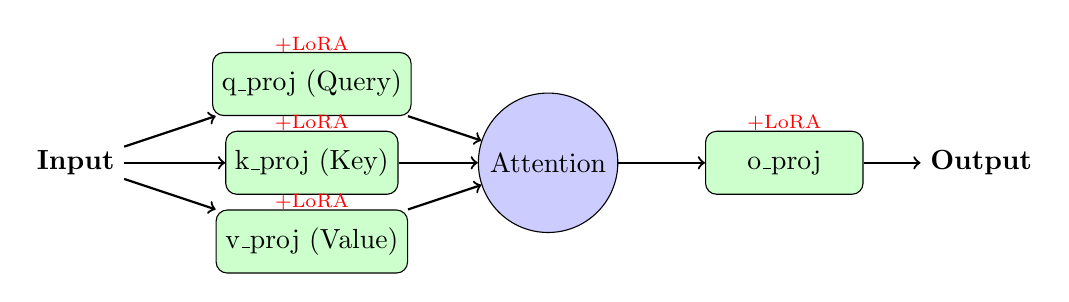
\begin{tikzpicture}[
    node distance=1cm,
    proj/.style={draw, rounded corners, minimum width=2cm, minimum height=0.8cm, fill=green!20},
    arrow/.style={->, thick}
]

% Input
\node (input) at (0,0) {\textbf{Input}};

% Projections
\node[proj] (q) at (3,1) {q\_proj (Query)};
\node[proj] (k) at (3,0) {k\_proj (Key)};
\node[proj] (v) at (3,-1) {v\_proj (Value)};

% Attention
\node[draw, circle, fill=blue!20, minimum size=1.5cm] (attn) at (6,0) {Attention};

% Output projection
\node[proj] (o) at (9,0) {o\_proj};

% Output
\node (output) at (11.5,0) {\textbf{Output}};

% Arrows
\draw[arrow] (input) -- (q);
\draw[arrow] (input) -- (k);
\draw[arrow] (input) -- (v);
\draw[arrow] (q) -- (attn);
\draw[arrow] (k) -- (attn);
\draw[arrow] (v) -- (attn);
\draw[arrow] (attn) -- (o);
\draw[arrow] (o) -- (output);

% LoRA labels
\node[text=red, font=\scriptsize] at (3,1.5) {+LoRA};
\node[text=red, font=\scriptsize] at (3,0.5) {+LoRA};
\node[text=red, font=\scriptsize] at (3,-0.5) {+LoRA};
\node[text=red, font=\scriptsize] at (9,0.5) {+LoRA};

\end{tikzpicture}
\caption{LoRA Adapters Applied to Attention Projections}
\end{figure}

\textbf{Why these modules?}
\begin{itemize}
    \item \textbf{q\_proj}: Controls what the model ``looks for'' - learns new query patterns
    \item \textbf{k\_proj}: Controls ``what information exists'' - improves context matching
    \item \textbf{v\_proj}: Controls ``what to output'' - modifies response content
    \item \textbf{o\_proj}: Controls ``how to combine'' - refines final representation
\end{itemize}

\subsection{ChatML Format}

The Qwen model uses ChatML format for conversations:

\begin{lstlisting}[language=Python, caption=ChatML Format Structure]
<|im_start|>system
You are a compassionate emotional support assistant.
Give warm, insightful responses about human emotions.
Keep answers concise (2-3 sentences) and end with a follow-up question.
<|im_end|>
<|im_start|>user
Why do I feel anxious even when everything is going well?
<|im_end|>
<|im_start|>assistant
Anxiety can appear even in good times because the brain sometimes scans 
for potential threats regardless of current circumstances. It's a 
protective mechanism that doesn't always match reality. What usually 
triggers that feeling for you?
<|im_end|>
\end{lstlisting}

\subsection{Configuration Parameters}

\begin{table}[H]
\centering
\caption{LoRA Configuration}
\begin{tabular}{lll}
\toprule
\textbf{Parameter} & \textbf{Value} & \textbf{Purpose} \\
\midrule
\texttt{r} (rank) & 16 & Controls adapter capacity \\
\texttt{lora\_alpha} & 32 & Scaling factor ($\alpha/r = 2.0$) \\
\texttt{lora\_dropout} & 0.1 & Prevents overfitting \\
\texttt{target\_modules} & [q,k,v,o]\_proj & All attention projections \\
\texttt{bias} & none & Don't train bias terms \\
\texttt{task\_type} & CAUSAL\_LM & Autoregressive generation \\
\bottomrule
\end{tabular}
\end{table}

\begin{table}[H]
\centering
\caption{Training Configuration}
\begin{tabular}{lll}
\toprule
\textbf{Parameter} & \textbf{Value} & \textbf{Rationale} \\
\midrule
Batch Size & 1 & Memory constraint on Mac \\
Gradient Accumulation & 4 & Effective batch = 4 \\
Learning Rate & 2e-4 & Standard for LoRA \\
Epochs & 2 & Prevent overfitting \\
Max Sequence Length & 256 & Sufficient for Q\&A \\
Optimizer & AdamW & Standard choice \\
Scheduler & Cosine & Smooth LR decay \\
Precision & FP16 & Memory efficient on MPS \\
\bottomrule
\end{tabular}
\end{table}

% ============================================
% SECTION 6: TRAINING PROCESS
% ============================================
\section{Training Process and Results}

\subsection{Training Progress}

\begin{figure}[H]
\centering
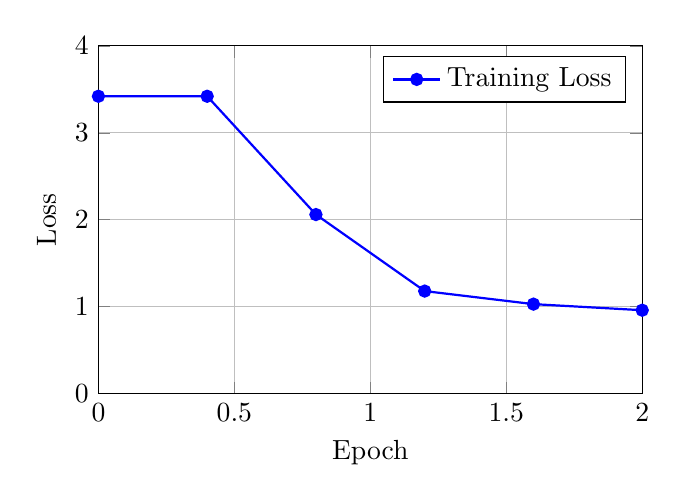
\begin{tikzpicture}
\begin{axis}[
    xlabel={Epoch},
    ylabel={Loss},
    xmin=0, xmax=2,
    ymin=0, ymax=4,
    legend pos=north east,
    grid=major,
    width=0.7\textwidth,
    height=6cm,
]
\addplot[
    color=blue,
    mark=*,
    thick,
] coordinates {
    (0, 3.42)
    (0.4, 3.42)
    (0.8, 2.06)
    (1.2, 1.18)
    (1.6, 1.03)
    (2.0, 0.96)
};
\addlegendentry{Training Loss}
\end{axis}
\end{tikzpicture}
\caption{Training Loss Curve Over 2 Epochs}
\end{figure}

\begin{figure}[H]
\centering
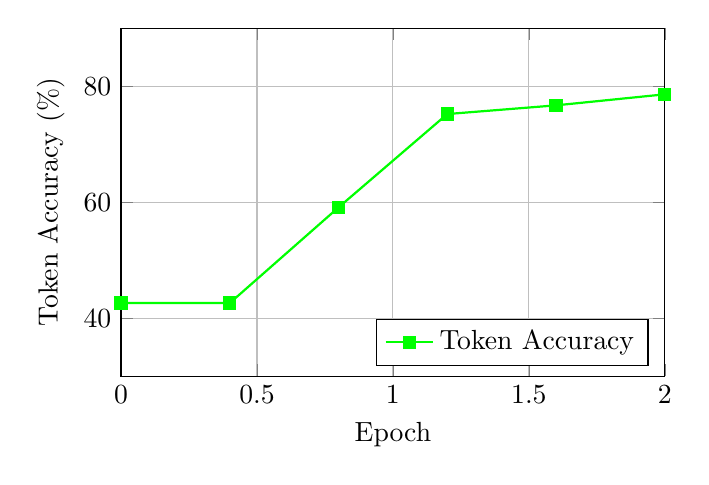
\begin{tikzpicture}
\begin{axis}[
    xlabel={Epoch},
    ylabel={Token Accuracy (\%)},
    xmin=0, xmax=2,
    ymin=30, ymax=90,
    legend pos=south east,
    grid=major,
    width=0.7\textwidth,
    height=6cm,
]
\addplot[
    color=green,
    mark=square*,
    thick,
] coordinates {
    (0, 42.6)
    (0.4, 42.6)
    (0.8, 59.1)
    (1.2, 75.2)
    (1.6, 76.7)
    (2.0, 78.6)
};
\addlegendentry{Token Accuracy}
\end{axis}
\end{tikzpicture}
\caption{Token Accuracy Improvement During Training}
\end{figure}

\subsection{Training Metrics Summary}

\begin{table}[H]
\centering
\caption{Training Results}
\begin{tabular}{lccc}
\toprule
\textbf{Metric} & \textbf{Start} & \textbf{End} & \textbf{Improvement} \\
\midrule
Loss & 3.42 & 0.96 & $\downarrow$ 72\% \\
Token Accuracy & 42.6\% & 78.6\% & $\uparrow$ 36 points \\
Learning Rate & 2e-4 & 5e-6 & Cosine decay \\
Training Time & \multicolumn{3}{c}{82.54 seconds} \\
\bottomrule
\end{tabular}
\end{table}

\subsection{What are Checkpoints?}

During training, the model saves intermediate states called \textbf{checkpoints}:

\begin{itemize}
    \item \textbf{checkpoint-48}: Saved after 48 training steps (end of epoch 1)
    \item \textbf{checkpoint-96}: Saved after 96 steps (end of epoch 2)
\end{itemize}

Checkpoints allow:
\begin{enumerate}
    \item Recovery if training crashes
    \item Comparing different training stages
    \item Selecting the best model (not just the final one)
\end{enumerate}

% ============================================
% SECTION 7: RESULTS AND COMPARISON
% ============================================
\section{Results: Base vs Fine-Tuned Model}

\subsection{Qualitative Comparison}

\textbf{Test Question:} \textit{``Why do I feel anxious even when everything is going well?''}

\begin{table}[H]
\centering
\caption{Model Output Comparison}
\small
\begin{tabular}{p{6cm}p{6cm}}
\toprule
\textbf{Base Model Response} & \textbf{Fine-Tuned Response} \\
\midrule
It's understandable to feel anxious sometimes! Here are some steps you can take to manage your anxiety:

1. \textbf{Deep Breathing}: Practice deep breathing exercises...

2. \textbf{Mindfulness}: Engage in mindfulness meditation...

3. \textbf{Physical Activity}: Exercise is great for reducing stress...

4. \textbf{Connect with Others}: Talk about how you're feeling...

5. \textbf{Routine}: Try maintaining a daily routine...
&
Anxiety can appear even in good times because the brain sometimes scans for potential threats regardless of current circumstances. It's a protective mechanism that doesn't always match reality. What usually triggers that feeling for you?
\\
\bottomrule
\end{tabular}
\end{table}

\subsection{Style Analysis}

\begin{figure}[H]
\centering
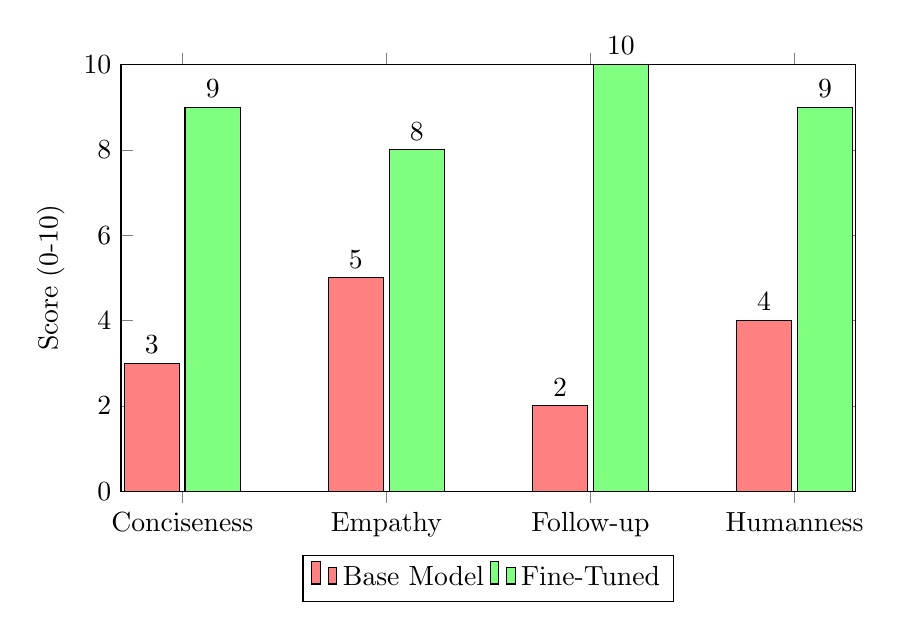
\begin{tikzpicture}
\begin{axis}[
    ybar,
    bar width=20pt,
    xlabel={Aspect},
    ylabel={Score (0-10)},
    ymin=0, ymax=10,
    symbolic x coords={Conciseness, Empathy, Follow-up, Humanness},
    xtick=data,
    nodes near coords,
    legend style={at={(0.5,-0.15)}, anchor=north, legend columns=2},
    width=0.9\textwidth,
    height=7cm,
]
\addplot[fill=red!50] coordinates {
    (Conciseness, 3)
    (Empathy, 5)
    (Follow-up, 2)
    (Humanness, 4)
};
\addplot[fill=green!50] coordinates {
    (Conciseness, 9)
    (Empathy, 8)
    (Follow-up, 10)
    (Humanness, 9)
};
\legend{Base Model, Fine-Tuned}
\end{axis}
\end{tikzpicture}
\caption{Qualitative Comparison of Model Outputs}
\end{figure}

\subsection{Key Differences}

\begin{table}[H]
\centering
\caption{Detailed Comparison}
\begin{tabular}{lcc}
\toprule
\textbf{Aspect} & \textbf{Base Model} & \textbf{Fine-Tuned} \\
\midrule
Response Length & Long (5 paragraphs) & Concise (3 sentences) \\
Format & Numbered lists & Natural prose \\
Tone & Clinical, instructional & Warm, conversational \\
Follow-up Question & None & Yes (always) \\
Personalization & Generic advice & Asks about user's experience \\
KnowSLM Compliance & No & Yes \\
\bottomrule
\end{tabular}
\end{table}

% ============================================
% SECTION 8: CODE DOCUMENTATION
% ============================================
\section{Code Documentation}

\subsection{Project Structure}

\begin{lstlisting}[language=bash, caption=Project Directory Structure]
assignment_2_open_elective/
|
|-- 2504.04569v2.pdf          # KnowSLM research paper
|
|-- emotions_dataset.csv       # 100 Q&A training pairs
|   +-- Columns: input, output
|
|-- train.py                   # Training script (~100 lines)
|   |-- Configuration section
|   |-- Data loading functions
|   |-- Model setup functions
|   +-- Training function
|
|-- test.py                    # Interactive testing script
|   |-- Model loading
|   |-- Generation function
|   +-- Interactive chat loop
|
|-- qwen_lora_adapter/         # Trained LoRA adapter
|   |-- adapter_config.json    # LoRA configuration
|   |-- adapter_model.safetensors  # Weights (~17 MB)
|   |-- tokenizer.json         # Tokenizer vocabulary
|   +-- tokenizer_config.json  # Tokenizer settings
|
|-- venv/                      # Python virtual environment
|
+-- report.tex                 # This report
\end{lstlisting}

\subsection{Training Script (train.py)}

\begin{lstlisting}[language=Python, caption=Key Training Code Snippets]
# LoRA Configuration
lora_config = LoraConfig(
    r=16,                    # Rank
    lora_alpha=32,           # Scaling factor
    lora_dropout=0.1,        # Dropout for regularization
    target_modules=["q_proj", "k_proj", "v_proj", "o_proj"],
    bias="none",
    task_type="CAUSAL_LM",
)

# Apply LoRA to model
model = get_peft_model(model, lora_config)

# Training configuration
training_config = SFTConfig(
    output_dir="./qwen_lora_adapter",
    per_device_train_batch_size=1,
    gradient_accumulation_steps=4,
    learning_rate=2e-4,
    num_train_epochs=2,
    max_length=256,
    fp16=True,  # For MPS
)

# Train
trainer = SFTTrainer(
    model=model,
    processing_class=tokenizer,
    train_dataset=dataset,
    args=training_config,
)
trainer.train()
\end{lstlisting}

\subsection{Testing Script (test.py)}

\begin{lstlisting}[language=Python, caption=Model Comparison Code]
# Load base model
base_model = AutoModelForCausalLM.from_pretrained(
    "Qwen/Qwen2.5-1.5B-Instruct",
    torch_dtype=torch.float16,
).to("mps")

# Load fine-tuned model
ft_model = AutoModelForCausalLM.from_pretrained(
    "Qwen/Qwen2.5-1.5B-Instruct",
    torch_dtype=torch.float16,
)
ft_model = PeftModel.from_pretrained(ft_model, "./qwen_lora_adapter")
ft_model = ft_model.to("mps")

# Generate and compare
print("[BASE]", generate(base_model, question))
print("[FINE-TUNED]", generate(ft_model, question))
\end{lstlisting}

% ============================================
% SECTION 9: USAGE INSTRUCTIONS
% ============================================
\section{Usage Instructions}

\subsection{Prerequisites}

\begin{itemize}
    \item Python 3.10+
    \item macOS with Apple Silicon (MPS) or Linux/Windows with CUDA
    \item $\sim$8 GB RAM minimum
\end{itemize}

\subsection{Installation}

\begin{lstlisting}[language=bash, caption=Setup Commands]
# Clone or navigate to project
cd assignment_2_open_elective

# Create virtual environment
python3 -m venv venv
source venv/bin/activate

# Install dependencies
pip install torch transformers datasets peft trl accelerate pandas
\end{lstlisting}

\subsection{Training}

\begin{lstlisting}[language=bash, caption=Training Command]
python train.py

# Expected output:
# Loaded 100 examples
# Trainable parameters: 4,358,144 (0.28%)
# Training... [progress bar]
# TRAINING COMPLETE! Adapter saved to: ./qwen_lora_adapter
\end{lstlisting}

\subsection{Testing}

\begin{lstlisting}[language=bash, caption=Testing Command]
python test.py

# Interactive session:
# Question: Why do I overthink everything?
# [BASE MODEL] ... (long response)
# [FINE-TUNED] ... (concise, empathetic response)
\end{lstlisting}

% ============================================
% SECTION 10: CONCLUSION
% ============================================
\section{Conclusion}

\subsection{Summary of Achievements}

\begin{enumerate}
    \item \textbf{Successfully fine-tuned} Qwen 2.5 1.5B using LoRA
    \item \textbf{Created synthetic dataset} following KnowSLM methodology
    \item \textbf{Achieved significant style adaptation} from generic to empathetic
    \item \textbf{Reduced training overhead} to 0.28\% of parameters
    \item \textbf{Documented entire process} for reproducibility
\end{enumerate}

\subsection{Key Learnings}

\begin{table}[H]
\centering
\caption{Key Learnings from the Project}
\begin{tabular}{p{4cm}p{8cm}}
\toprule
\textbf{Topic} & \textbf{Insight} \\
\midrule
LoRA & Enables fine-tuning on consumer hardware by training only 0.28\% of parameters \\
Dataset Quality & Format and style matter more than quantity for style adaptation \\
KnowSLM & Follow-up questions significantly improve conversation naturalness \\
Evaluation & Side-by-side comparison clearly shows style improvements \\
\bottomrule
\end{tabular}
\end{table}

\subsection{Limitations}

\begin{itemize}
    \item Small dataset (100 examples) limits generalization
    \item Some responses may still echo training data patterns
    \item KnowSLM paper suggests 500+ examples for robust improvement
\end{itemize}

\subsection{Future Improvements}

\begin{enumerate}
    \item Expand dataset to 500+ examples
    \item Add more diverse emotional topics
    \item Implement LLM-judge evaluation from KnowSLM
    \item Try RAG augmentation for factual accuracy
    \item Experiment with different LoRA ranks
\end{enumerate}

% ============================================
% REFERENCES
% ============================================
\begin{thebibliography}{9}

\bibitem{knowslm}
Harbola, C., \& Purwar, A. (2025).
\textit{KnowSLM: A framework for evaluation of small language models for knowledge augmentation and humanised conversations}.
arXiv:2504.04569.

\bibitem{hu2021lora}
Hu, E. J., et al. (2021).
\textit{LoRA: Low-Rank Adaptation of Large Language Models}.
arXiv:2106.09685.

\bibitem{qwen}
Qwen Team. (2024).
\textit{Qwen2.5 Technical Report}.
Alibaba Cloud.

\bibitem{peft}
Mangrulkar, S., et al. (2023).
\textit{PEFT: State-of-the-art Parameter-Efficient Fine-Tuning methods}.
GitHub: huggingface/peft.

\bibitem{trl}
von Werra, L., et al. (2023).
\textit{TRL: Transformer Reinforcement Learning}.
GitHub: huggingface/trl.

\end{thebibliography}

% ============================================
% APPENDIX
% ============================================
\appendix
\section{Complete Training Script}

\lstinputlisting[language=Python, caption=train.py - Complete Code]{train.py}

\section{Complete Testing Script}

\lstinputlisting[language=Python, caption=test.py - Complete Code]{test.py}

\end{document}
